\documentclass{BHCexam}
\begin{document}
\biaoti{三角函数}
\fubiaoti{}
\maketitle
\tableofcontents
\begin{questions}

\section{选择}
\qs 已知$\sin 2\alpha=\dfrac{2}{3}$,则$\cos^2\left(\alpha+\dfrac{\pi}{4}\right)=$\xx
\onech{$\dfrac{1}{6}$}{$\dfrac{1}{3}$}{$\dfrac{1}{2}$}{$\dfrac{2}{3}$}
\qs 若$ \sin \left(\dfrac{\pi}{6}-\alpha\right)=\dfrac{1}{3},~ $则$ \cos \left(\dfrac{2\pi}{3}+2\alpha\right)= $\xx
\onech{$ -\dfrac{7}{9}$}{$ -\dfrac{1}{3}$}{$ \dfrac{1}{3}$}{$ \dfrac{7}{9}$}
\qs 若$ \tan \theta+\dfrac{1}{\tan \theta} =4,~$则$ \sin 2\theta =$\xx
\onech{$ \dfrac{1}{5}$}{$ \dfrac{1}{4}$}{$ \dfrac{1}{3}$}{$ \dfrac{1}{2}$}
\qs 函数$f(x)=\cos\left(\omega x+\varphi\right)$的部分图象如图所示,则$f(x)$的单调递减区间为\xx\begin{center}
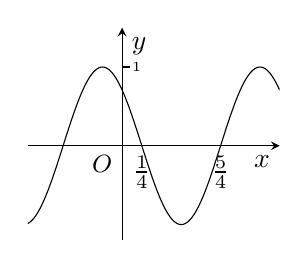
\begin{tikzpicture}
\node[below left](O) at(0,0) {\small$\bm{O}$};
\draw(0,1)node[right]{\tiny$1$}--(0.1,1);
\clip(-1.2,-1.2) rectangle (2,1.5);
\draw[->,>=stealth](-1.2,0)--(2,0) node[below left] (x){$x$};
\draw[->,>=stealth](0,-1.2)--(0,1.5) node[below right] (y){$y$};
\draw[domain=-1.2:2,samples=1000] plot(\x,{cos((pi*(\x)+1/4*pi) r)});
\node[below] (A)at (0.25,0){$\frac{1}{4}$};
\node[below] (B)at (1.25,0){$\frac{5}{4}$};
\end{tikzpicture}
\end{center}
\twochx{$ \left(k\pi-\dfrac{1}{4},k\pi+\dfrac{3}{4}\right),k\inZ$}{$ \left(2k\pi-\dfrac{1}{4},2k\pi+\dfrac{3}{4}\right),k\inZ$}{$ \left(k-\dfrac{1}{4},k+\dfrac{3}{4}\right),k\inZ$}{$\left(2k-\dfrac{1}{4},2k+\dfrac{3}{4}\right),k\inZ $}

\question 设$\alpha \in \left(0,\dfrac{\pi}{2}\right),\beta \in \left(0,\dfrac{\pi}{2}\right)$,且$\tan \alpha =\dfrac{1+\sin \beta}{\cos \beta}$,则\xx
\twoch{$3\alpha-\beta=\dfrac{\pi}{2}$}{$3\alpha+\beta=\dfrac{\pi}{2}$}{$2\alpha-\beta=\dfrac{\pi}{2}$}{$2\alpha+\beta=\dfrac{\pi}{2}$}
\question 函数$f(x)=\cos 2x+6\cos \left(\dfrac{\pi}{2}-x\right)$的最大值为\xx
\onech{4}{5}{6}{7}

\qs 将函数$ y=\sin\left(2x+\dfrac{\pi}{3}\right) $图象上的点$ P\left(\dfrac{\pi}{4},t\right) $向左平移$ s~(s>0) $个单位长度得到点$ P' $.若$ P' $位于函数 $ y=\sin 2x $的图象上,则\xx
\twochx{$ t=\dfrac{1}{2},~s\text{的最小值为}\dfrac{\pi}{6} $}{$ t=\dfrac{\sqrt{3}}{2},~s\text{的最小值为}\dfrac{\pi}{6} $}{$ t=\dfrac{1}{2},~s\text{的最小值为}\dfrac{\pi}{3} $}{$ t=\dfrac{\sqrt{3}}{2},~s\text{的最小值为}\dfrac{\pi}{3} $}
\question 已知函数$f(x)=\sin(\omega x+\varphi)~\left(\omega>0,\abs{\varphi}\le \dfrac{\pi}{2}\right),x=-\dfrac{\pi}{4}$为$f(x)$的零点,$x=\dfrac{\pi}{4}$为$y=f(x)$图象的对称轴,且$f(x)$在$\left(\dfrac{\pi}{18},\dfrac{5\pi}{36}\right)$单调,则$\omega$的最大值为\xx
\onech{11}{9}{7}{5}
\qs 已知$ \omega>0,~ $函数$f(x)=\sin (\omega x+\dfrac{\pi}{4})$在$\left(\dfrac{\pi}{2},\pi\right)  $上单调递减,则$ \omega $的取值范围是\xx
\onech{$ \left[\dfrac{1}{2},\dfrac{5}{4}\right] $}{$ \left[\dfrac{1}{2},\dfrac{3}{4}\right] $}{$ \left(0,\dfrac{1}{2}\right] $}{$ \left(0,2\right] $}
\qs 已知$ \omega>0,~0<\varphi <\pi,~ $直线$ x=\dfrac{\pi}{4} $和$ x=\dfrac{5\pi}{4} $是函数$f(x)=\sin (\omega x+\varphi)$的图象的两条相邻对称轴,则$ \varphi= $\xx
\onech{$ \dfrac{\pi}{4} $}{$ \dfrac{\pi}{3} $}{$ \dfrac{\pi}{2} $}{$ \dfrac{3\pi}{4} $}

\qs 将函数$f(x)=\sin (2x+\theta)\left(-\dfrac{\pi}{2}<\theta<\dfrac{\pi}{2}\right)$的图象向右平移$ \varphi(\varphi>0) $个单位长度后得到函数$g(x)$的图象,若$f(x),~g(x)$的图象都经过点$ P\left(0,\dfrac{\sqrt{3}}{2}\right) $,~则$ \varphi $的值可以是\xx
\onech{$ \dfrac{5\pi}{3}$}{$ \dfrac{5\pi}{6}$}{$ \dfrac{\pi}{2}$}{$ \dfrac{\pi}{6}$}
\qs 已知函数$f(x)=2\sin \left(\omega x+\varphi\right),~x \inR$,~其中$ \omega>0,~-\pi <\varphi\le \pi ,~ $若$f(x)$的最小正周期为$ 6\pi  $,且当$ x=\dfrac{\pi}{2} $时,$f(x)$取得最大值,则\xx
\twoch{$f(x)$在区间$ \left[-2\pi,0\right] $上是增函数}{$f(x)$在区间$ \left[-3\pi,-\pi \right] $上是增函数}{$f(x)$在区间$ \left[3\pi,5\pi \right] $上是减函数}{$f(x)$在区间$ \left[4\pi,6\pi \right] $上是减函数}

\qs 已知函数$f(x)=\sin (\omega x +\varphi)+\cos (\omega x+\varphi)~\left(\omega>0,\left|\varphi\right|<\dfrac{\pi}{2}\right)$的最小正周期为$ \pi ,~ $且$ f(-x)=f(x),~ $则\xx
\twoch{$ f(x) $在$ \left(0,\dfrac{\pi}{2}\right) $上单调递减}{$ f(x) $在$ \left(\dfrac{\pi}{4},\dfrac{3\pi}{4}\right) $上单调递减}{$ f(x) $在$ \left(0,\dfrac{\pi}{2}\right) $上单调递增}{$ f(x) $在$ \left(\dfrac{\pi}{4},\dfrac{3\pi}{4}\right) $上单调递增}


\qs 在$\triangle ABC$中,$ \angle A=\dfrac{\pi}{3},~BC=3 $,则$ \triangle ABC $的周长为\xx
\twoch{$ 4\sqrt{3}\sin \left(B+\dfrac{\pi}{3}\right)+3$}{$4\sqrt{3}\sin \left(B+\dfrac{\pi}{6}\right)+3 $}{$6\sin \left(B+\dfrac{\pi}{3}\right)+3 $}{$ 6\sin \left(B+\dfrac{\pi}{6}\right)+3$}
\qs $\triangle ABC$的内角$ A,~B,~C $所对的边分别为$ a,b,c $.若$ a\sin A\sin B+b\cos^2A=\sqrt{2}a,~ $则$ \dfrac{b}{a}=$\xx
\onech{$ 2\sqrt{3}$}{$ 2\sqrt{2}$}{$ \sqrt{3}$}{$ \sqrt{2}$}
\qs 在$ \triangle ABC $中,若$ \sin ^2A+\sin^2 B<\sin ^2C $,则$ \triangle ABC $的形状是\xx
\onech{钝角三角形}{直角三角形}{锐角三角形}{不能确定}
\qs 已知锐角$\triangle ABC$的内角$A,B,C$的对边分别为$a,b,c$,$23\cos^2A+\cos 2A=0$,$a=7$,$c=6$,则$b=$\xx
\onech{10}{9}{8}{5}
\qs 设$\triangle ABC$中,$ A,B,C $所对的边分别为$ a,b,c $,若三边的长为连续的三个正整数,且$ A>B>C ,~3b=20 a\cos A$,则$ \sin A:\sin B:\sin C =\xx$
\onech{$ 4:3:2$}{$ 5:6:7$}{$ 5:4:3$}{$ 6:5:4$}
\section{填空}
\qs 设$\theta$为第二象限角,若$ \tan\left(\theta +\dfrac{\pi}{4}\right)=\dfrac{1}{2},~ $则$ \sin \theta+\cos \theta $=\tk.

\qs 已知$\sin \alpha=\dfrac{1}{2}+\cos \alpha,~$且$ \alpha\in \left(0,\dfrac{\pi}{2}\right),~ $则$ \dfrac{\cos 2\alpha}{\sin \left(\alpha-\dfrac{\pi}{4}\right)} $的值为\tk.
\question 函数$f(x)=\sin (x+2\varphi)-2\sin \varphi \cos(x+\varphi)$的最大值为\tk.
\question 设当$x=\theta$时,函数$f(x)=\sin x-2\cos x$取得最大值,则$\cos \theta=$\tk.

\qs 已知函数$f(x)=2\sin \omega x~(\omega>0)$在区间$ \left[-\dfrac{\pi}{3},\dfrac{\pi}{4}\right] $上的最小值是$ -2 $,则$ \omega $的最小值是\tk.
\qs 设函数$ f(x)=A\sin (\omega x+\varphi)~(A,\omega,\varphi \text{是常数,}A>0,\omega>0)$.若$ f(x) $在区间$ \left[\dfrac{\pi}{6},\dfrac{\pi}{2}\right] $上具有单调性,且$f(\dfrac{\pi}{2})=f(\dfrac{2\pi}{3})=-f(\dfrac{\pi}{6}) $,则$ f(x) $的最小正周期是\tk.\qs 将函数$f(x)=\sin (\omega x+\varphi)~\left(\omega >0,-\dfrac{\pi}{2}\le \varphi< \dfrac{\pi}{2}\right)$图像上每个点的横坐标缩短为原来的一半,纵坐标不变,再向右平移$ \dfrac{\pi}{6} $个单位长度得到$ y=\sin x $的图象,则$ f\left(\dfrac{\pi}{6}\right) $=\tk.
\qs 已知点$ A\left(\dfrac{\pi}{6},\dfrac{\sqrt{3}}{2}\right),~B\left(\dfrac{\pi}{4},1\right),~C\left(\dfrac{\pi}{2},0\right)$,若这三个点中有且仅有两个点在函数$f(x)=\sin \omega x$的图象上,则\CJKunderdot{正数}$ \omega $的最小值为\tk.

\qs 函数$y=\cos (2x+\varphi)~(-\pi<\varphi<\pi)$的图象向右平移$\dfrac{\pi}{2}$个单位后,与函数$y=\sin (2x+\dfrac{\pi}{3})$的图象重合,则$\varphi=$\tk.
\qs 在平面直角坐标系$xOy$中,角$ \alpha $与角$ \beta $均以$ Ox $为始边,它们的终边关于$y$轴对称.若$ \sin \alpha=\dfrac{1}{3}, $则$ \cos\left(\alpha-\beta\right)=\tk $.
\qs 把函数$ y=\sin 2x $的图象沿$x$轴向左平移$ \dfrac{\pi}{6} $个单位,纵坐标伸长到原来的2倍(横坐标不变)后得到函数$ y=f(x) $的图象,对于函数$ y=f(x) $有以下四个判断:\\
\ding{192} 该函数的解析式为$ y=2\sin \left(2x+\dfrac{\pi}{6}\right) $;\\
\ding{193} 该函数图象关于点$ \left(\dfrac{\pi}{3},0\right) $对称;\\
\ding{194} 该函数在$ \left[0,\dfrac{\pi}{6}\right] $上是增函数;\\
\ding{195} 若函数$ y=f(x)+a $在$ \left[0,\dfrac{\pi}{2}\right] $上的最小值为$ \sqrt{3},~ $则$ a=2\sqrt{3} .$\\
其中,正确判断的序号是\tk.




\qs 在三角形$\triangle ABC$中,$ B=60^{\circ} $,$ AC=\sqrt{3} $,则$ AB+2BC $的最大值为\tk.


\qs 在三角形$\triangle ABC$中,$ a=3,b=\sqrt{6} $,$ \angle A=\dfrac{2\pi}{3} $,则$ \angle B= $\tk.

\qs 在三角形$\triangle ABC$中,若$ a=2,~b+c=7,~\cos B=-\dfrac{1}{4} $,则$ b= $\tk.

\qs 在三角形$\triangle ABC$中,$ a=4,b=5,c=6 $,则$ \dfrac{\sin 2A}{\sin C}=$\tk.
\qs 若$\triangle ABC$的内角满足$ \sin A+\sqrt{2}\sin B=2\sin C $,则$ \cos C $的最小值是\tk.
\question 在平面四边形$ABCD$中,$\angle A=\angle B=\angle C=75^{\circ},~$$ BC=2,~ $则$AB$的取值范围是\tk.
\qs 在$\triangle ABC$中,$ D $为$ BC $边上的一点,$ BC=3BD,~AD=\sqrt{2},~\angle ADB=135^{\circ}.~ $若$ AC=\sqrt{2}AB $,则$ BD= $\tk.
\question 已知$a,~b,~c$分别为$\triangle ABC$三个内角$A$,~$B$,~$C$的对边,$a=2$,且$(2+b)(\sin A-\sin B)=(c-b)\sin C$,则$\triangle ABC$面积的最大值为\tk.
\section{简答题}
\qs $\triangle ABC$的内角$ A,~B,~C $的对边分别为$ a,~b,~c $,已知$ \bm{\triangle}ABC $的面积为$ \dfrac{a^2}{3\sin A} $.
\begin{parts}
\part 求$ \sin B\sin C $;
\part 若$ 6\cos B \cos C=1,~a=3 $,求$\bm{\triangle} ABC$的周长.
\end{parts}
\newpage
\qs $\triangle ABC$的内角$ A,~B,~C $的对边分别为$ a,~b,~c $,已知$ \sin A+\sqrt{3}\cos A =0,~a=2\sqrt{7},~b=2.$
\begin{parts}
\part 求$ c $;
\part 设$ D $为$ BC $边上的一点,且$ AD\bm{\bot}AC $,求$ \triangle ABD $的面积.
\end{parts}
\kongbai
\qs $\triangle ABC$的内角$ A,~B,~C $的对边分别为$ a,~b,~c $,已知$ \sin\left(A+C\right) =8\sin^2\dfrac{B}{2}$.
\begin{parts}
\part 求$ \cos B $;
\part 若$ a+c=6,~\triangle ABC$的面积为$ 2, ~$求$ b .$
\end{parts}
\kongbai
\qs 已知函数$f(x)=\sqrt{3}\cos\left(2x-\dfrac{\pi}{3}\right)-2\sin x\cos x$.
\begin{parts}
\part 求$f(x)$的最小正周期;
\part 求证:当$ x\in\left[-\dfrac{\pi}{4},\dfrac{\pi}{4}\right] $时,$f(x)\ge -\dfrac{1}{2}$.
\end{parts}
\kongbai
\qs 在$\triangle ABC$中,$ \angle A=60^{\circ},c=\dfrac{3}{7}a. $
\begin{parts}
\part 求$ \sin C $的值;
\part 若$ a=7 $,求$\triangle ABC$的面积.
\end{parts}
\kongbai
\qs 已知$a,b,c$分别为$\triangle ABC$内角$A,B,C$的对边,$\sin^2B=2\sin A\sin C$.
\begin{parts}
\part 若$a=b$,求$\cos B$;
\part 若$B=90^{\circ}$,且$a=\sqrt{2}$,求$\triangle ABC$的面积.
\end{parts}
\newpage
\qs 在$ \bm{\triangle} ABC $中,$ a^2+c^2=b^2+\sqrt{2}ac $.
\begin{parts}
\part 求$ \angle B $的大小;
\part 求$ \sqrt{2}\cos A+\cos C $的最大值.
\end{parts}
\kongbai
\qs 已知函数$f(x)=2\sin \omega x\cos \omega x+\cos 2\omega x (\omega >0) $的最小正周期为$ \pi $.
\begin{parts}
\part 求$ \omega $的值;
\part 求$ f(x) $的单调递增区间.
\end{parts}
\newpage
\qs 已知函数$f(x)=\sqrt{2}\sin \dfrac{x}{2}\cos \dfrac{x}{2}-\sqrt{2}\sin^2 \dfrac{x}{2}$.
\begin{parts}
\part 求$ f(x) $的最小正周期
\part 求$ f(x) $在区间$\left[-\pi,0\right]$上的最小值.
\end{parts}
\kongbai
\qs 已知函数$f(x)=\sin x-2\sqrt{3}\sin^2 \dfrac{x}{2}$.
\begin{parts}
\part 求$ f(x)  $的最小正周期;
\part 求$ f(x) $在区间$ \left[0,\dfrac{2\pi}{3}\right] $上的最小值.
\end{parts}
\newpage
\qs $\triangle ABC$的内角$ A,B,C $的对边$ a,b,c ~$.已知$ 2\cos C(a\cos B +b \cos A)=c $.
\begin{parts}
\part 求$ C $;
\part 若$ c=\sqrt{7} $,$ \triangle ABC $的面积为$ \dfrac{3\sqrt{3}}{2} $,求$ \triangle ABC $的周长.
\end{parts}
\kongbai
\qs 如图,在三角形$\triangle ABC$中,$ \angle B=\dfrac{\pi}{3} $,$~ AB=8 $,点$ D $在$ BC $边上,且$ CD=2 $,$ \cos \angle ADC=\dfrac{1}{7} $
\begin{parts}
\part 求$ \sin \angle BAD $;
\part 求$ BD,AC $的长.
\end{parts}
\vspace{-4em}\mbox{\hspace{1pt}}\hfill
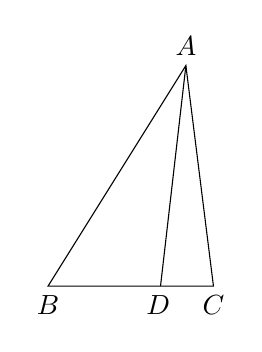
\begin{tikzpicture}[x=0.7cm, y=0.7cm]
\draw (0,0) node[below ](B){$B$}--(2,0) node[below] (D) {$D$}--(3,0)node[below] (C) {$C$}--(2.5,4) node[ above] (A) {$A$}--cycle;
\draw (2.5,4)--(D);
\end{tikzpicture}
\newpage
\qs 已知函数$f(x)=(2\cos^2 x-1)\sin 2x+\dfrac{1}{2}\cos 4x$
\begin{parts}
\part 求$ f(x) $的最小正周期及最大值;
\part 若$ \alpha \in \left(\dfrac{\pi}{2},\pi \right) $,且$ f(\alpha )=\dfrac{\sqrt{2}}{2} $,求$ \alpha $的值.
\end{parts}
\kongbai
\qs
已知函数$f(x)=4\cos x\sin (x+\dfrac{\pi}{6})-1.$
\begin{parts}
\part 求$ f(x) $的最小正周期
\part 求$ f(x) $在区间$ \left[-\dfrac{\pi}{6},\dfrac{\pi}{4}\right] $上的最大值和最小值.
\end{parts}
\kongbai 
\qs 已知函数$f(x)=2\cos 2x+\sin^2 x-4\cos x$.
\begin{parts}
\part 求$ f(\dfrac{\pi}{3}) $的值;
\part 求$ f(x) $的最大值和最小值.
\end{parts}
\kongbai
\qs 在三角形$\triangle ABC$中,内角$ A,~B,~C,~ $对边的边长分别是$ a,~b,~c ,~$已知$ c=2,C=\dfrac{\pi}{3} .$
\begin{parts}
\part 若三角形$\triangle ABC$的面积等于$\sqrt{3},~ $求$ a,b $;
\part 若$ \sin C+\sin (B-A)=2\sin 2A,~ $求$ \triangle ABC $的面积.
\end{parts}
\kongbai
\qs 已知函数$f(x)=\sin^2 \omega x+2\sqrt{3}\sin \omega x\bm{\cdot}\cos \omega x-\cos^2 \omega x+\lambda$的图象关于直线$ x=\pi $对称,其中$ {\omega ,\lambda} $为常数,且$ \omega \in \left(\dfrac{1}{2},1\right). $
\begin{parts}
\part 求函数$f(x)$的最小正周期;
\part 若$ y=f(x) $的图象经过点$ \left(\dfrac{\pi}{4},0\right),~ $求函数$f(x)$的值域.
\end{parts}
\kongbai
\qs 在三角形$\triangle ABC$中,角$A,~B,~C,~$所对的边长分别是$a,~b,~c,~$且$ a\cos B=3,~b\sin A=4. $
\begin{parts}
\part 求边长$ a; $
\part 若三角形$\triangle ABC$的面积$ S=10,~ $求$ \triangle ABC $的周长$ l. $
\end{parts}
\kongbai
\qs 在三角形$\triangle ABC$中,角$A,~B,~C,~$所对的边长分别是$a,~b,~c,~$已知$ \cos C+(\cos A-\sqrt{3}\sin A)\cos B=0. $
\begin{parts}
\part 求角$ B $的大小;
\part 若$ a+c=1,~ $求$ b $的取值范围.
\end{parts}
\kongbai
\qs 在锐角三角形$\triangle ABC$中,角$A,~B,~C,~$所对的边长分别是$a,~b,~c,~$,且$ \sqrt{3}a=2c\sin A $
\begin{parts}
\part 确定角$ C $的大小;
\part 若$ c=\sqrt{7},~ $且三角形$\triangle ABC$的面积为$ \dfrac{3\sqrt{3}}{2},~ $求$ a+b $的值.
\end{parts}
\newpage
\qs 四边形$ ABCD $ 的内角$ A $与$ C $互补,$ AB=1,~BC=3,~CD=DA=2. $
\begin{parts}
\part 求$ C $和$ BD $;
\part 求四边形$ ABCD $的面积.
\end{parts}

\kongbai
\qs 在三角形$\triangle ABC$中,角$A,~B,~C,~$所对的边长分别是$a,~b,~c,~$已知$ A=\dfrac{\pi}{4},~b\sin (\dfrac{\pi}{4}+C)-c\sin (\dfrac{\pi}{4}+B)=a. $求证:$ B-C=\dfrac{\pi}{2}. $

\newpage
\qs $\triangle ABC$中的内角$ A,~B,~C $的对边分别为$ a,~b,~c,~ $已知$ a=b\cos C+c\sin B $.
\begin{parts}
\part 求$ B $;
\part 若$ b=2 $,求$\triangle ABC$面积的最大值.
\end{parts}
\kongbai
\qs 在$\triangle ABC$中,内角$ A,~B,~C $的对边长分别为$ a,~b,~c $,已知$ a^2-c^2=2b $,且$ \sin B=4\cos A\sin C $,求$ b $.
\newpage
\qs 在三角形$\triangle ABC$中,角$A,~B,~C,~$所对的边长分别是$a,~b,~c,~$已知$ \cos (A-C)+\cos B=1,~a=2c, $求$ C $.
\end{questions}
\end{document}